\section{Prototype work}
For this sprint, we have refactored a few of the older prototypes and also created some new ones for the new user stories.

\subsection{New timer and weekplan template}
We refactored the timer on the show activity screen to use the common Giraf buttons so that we can keep a consistent design. The figure to the right shows a screen for selecting a template when creating a new weekplan.
\begin{figure}[H]
    \begin{subfigure}{0.5\textwidth}
    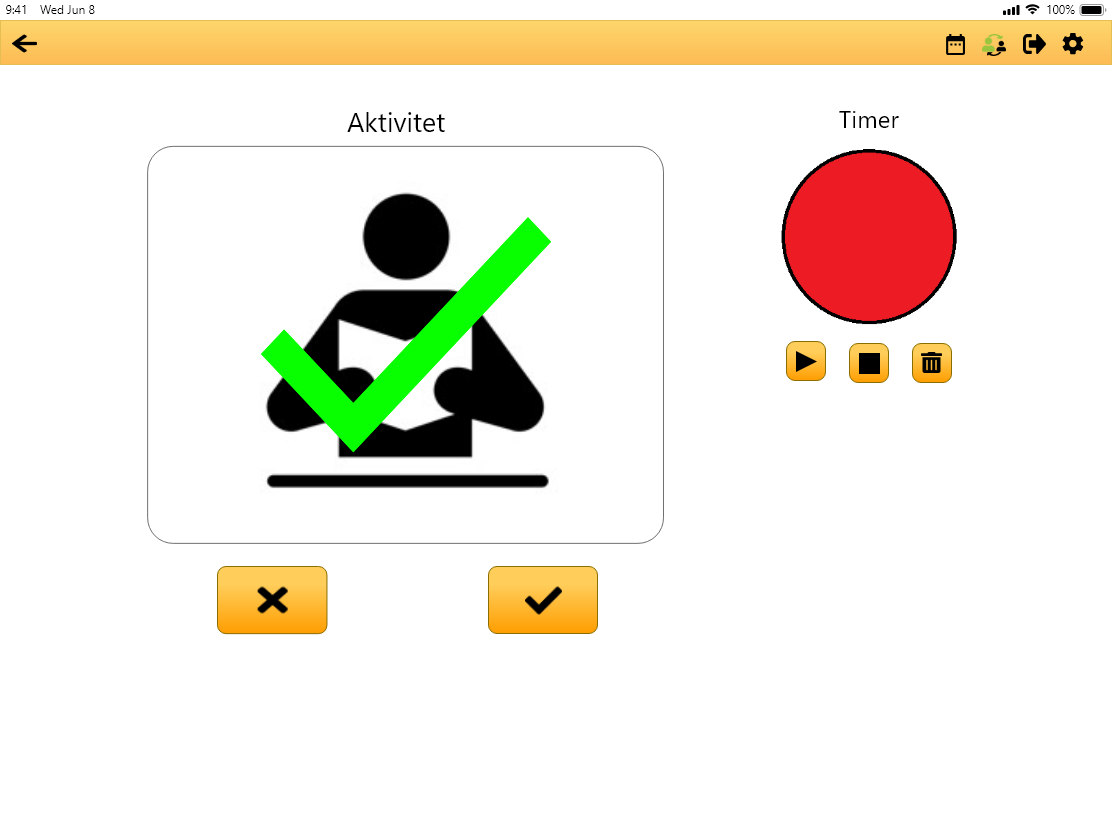
\includegraphics[width=1\linewidth, height=5cm]{sprint3-prototypes/aktivitet_new_timer.png} 
    \caption{New timer for activity}
    \label{fig:activity_new_timer}
    \end{subfigure}
    \begin{subfigure}{0.5\textwidth}
        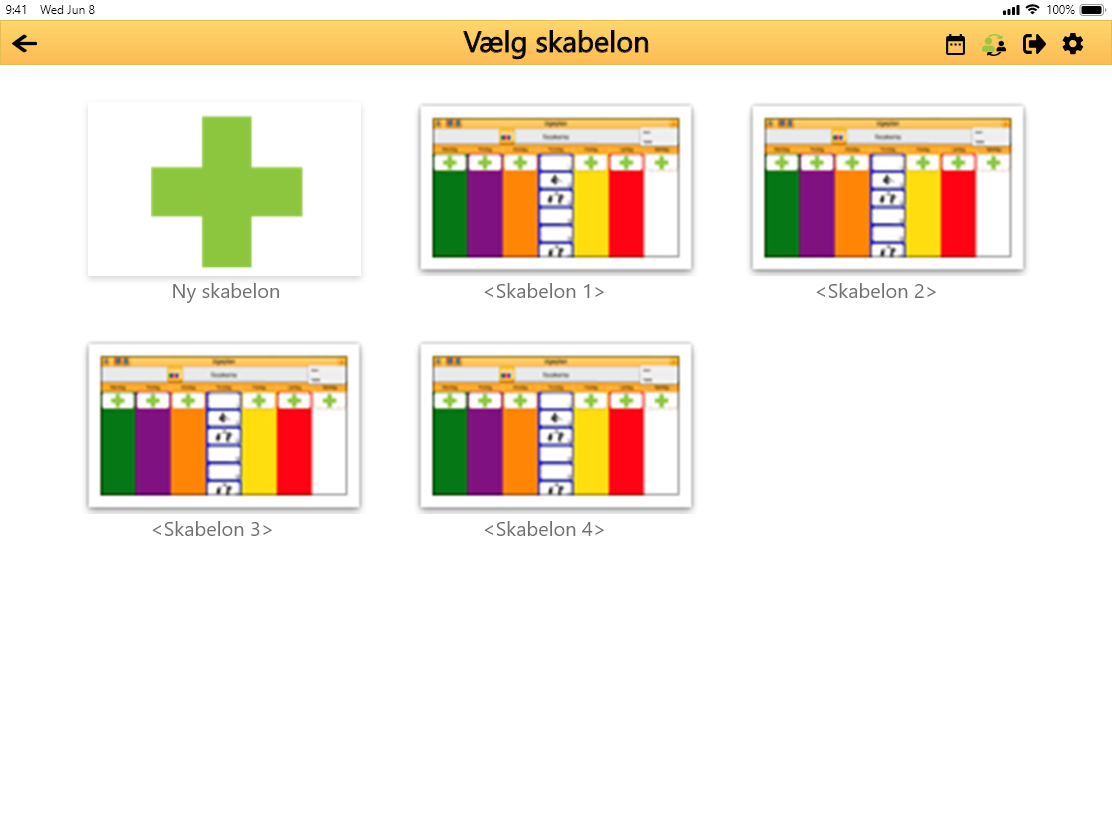
\includegraphics[width=1\linewidth, height=5cm]{sprint3-prototypes/ugeplan_skabelon.png}
    \caption{Weekplan template select screen}
    \label{fig:weekplan_template_screen}
    \end{subfigure} 
\end{figure}

\subsection{Setting pages}
We created a number of prototypes for the settings pages. Here we show two of them where the first is the overall view of the settings, and the on second one shows the settings screen where the guardian can select a color theme for the weekplan.
\begin{figure}[H]
    \begin{subfigure}{0.5\textwidth}
    \includegraphics[width=1\linewidth, height=5cm]{sprint3-prototypes/indstillinger.png} 
    \caption{Setting page}
    \label{fig:settings}
    \end{subfigure}
    \begin{subfigure}{0.5\textwidth}
        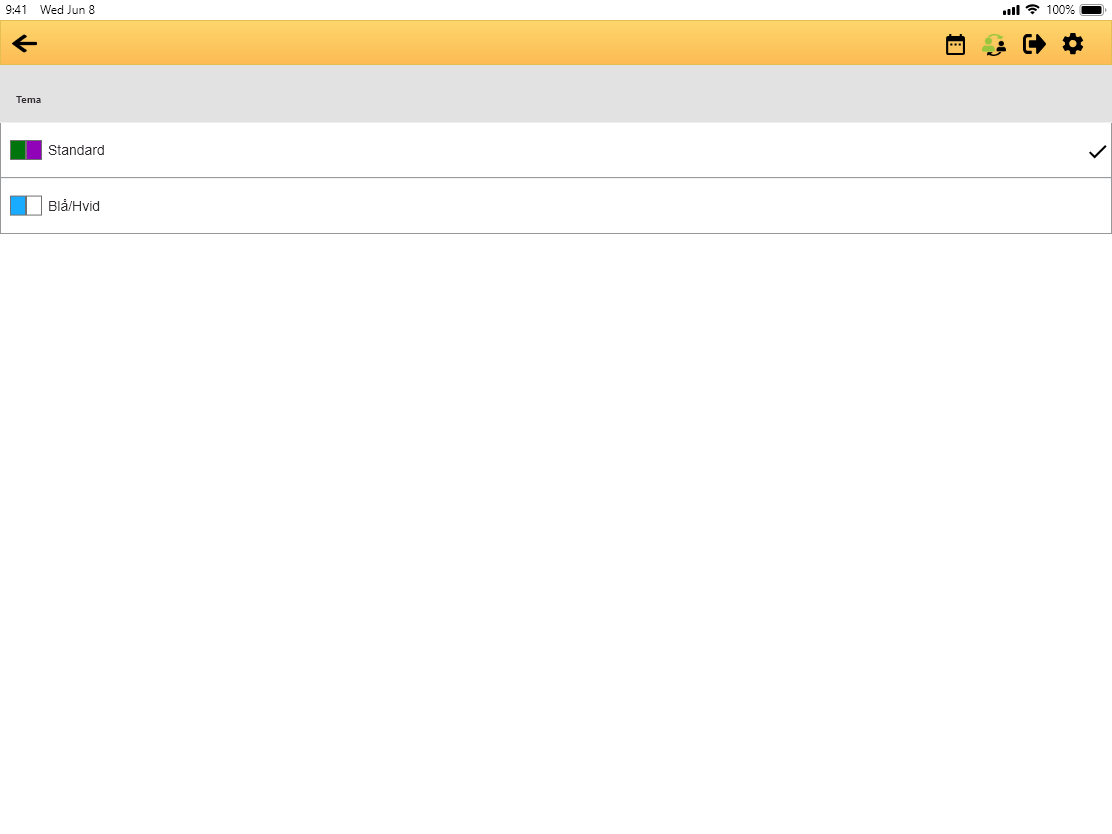
\includegraphics[width=1\linewidth, height=5cm]{sprint3-prototypes/indstillinger_ugeplan_farver.png}
    \caption{Settings page for weekplan color choice}
    \label{fig:settings_color_choice}
    \end{subfigure} 
\end{figure}

\subsection{Copy weekplan}
We refactored the prototypes for copying a weekplan to other citizens to include the new dialog boxes to make the design consistent. In \autoref{fig:copy_weekplan} we see a confirm dialog for copying a weekplan. In \autoref{fig:copy_weekplan_confirm_copy} we see the screen for choosing which citizens the weekplan should be copied to. 
\begin{figure}[H]
    \begin{subfigure}{0.5\textwidth}
    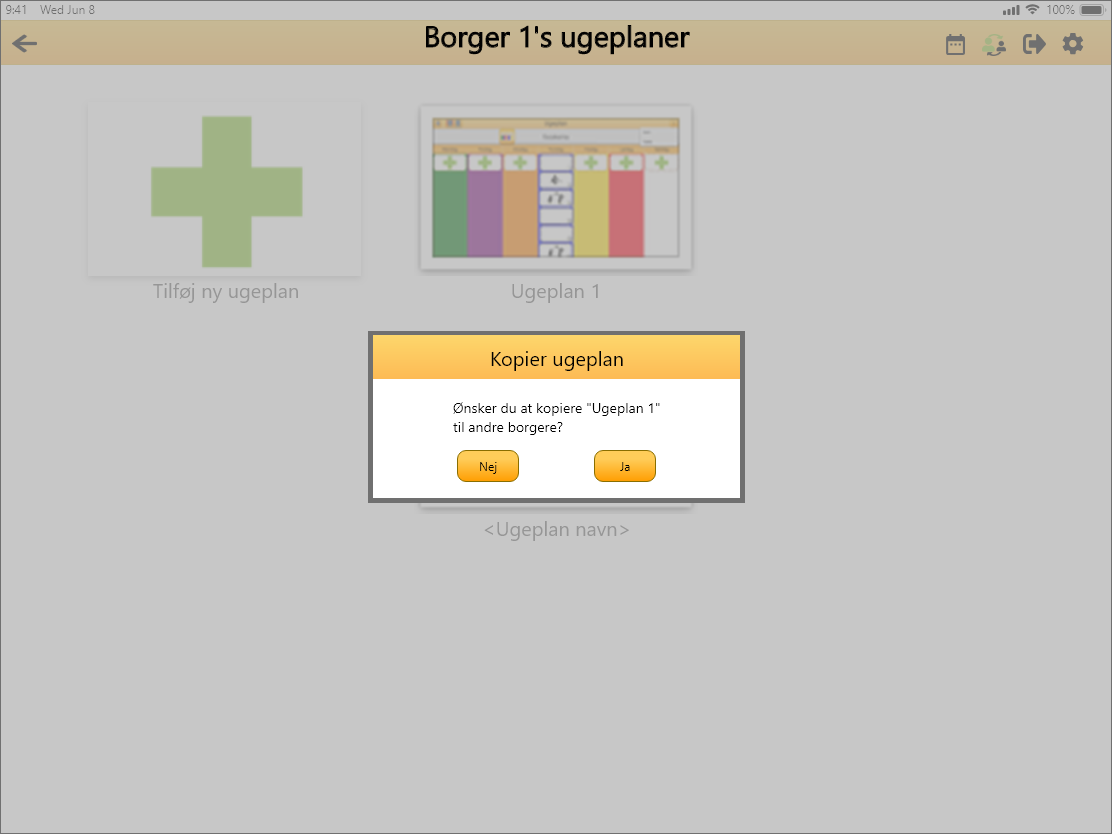
\includegraphics[width=1\linewidth, height=5cm]{sprint3-prototypes/copy_weekplan.png} 
    \caption{Copy weekplan dialog}
    \label{fig:copy_weekplan}
    \end{subfigure}
    \begin{subfigure}{0.5\textwidth}
        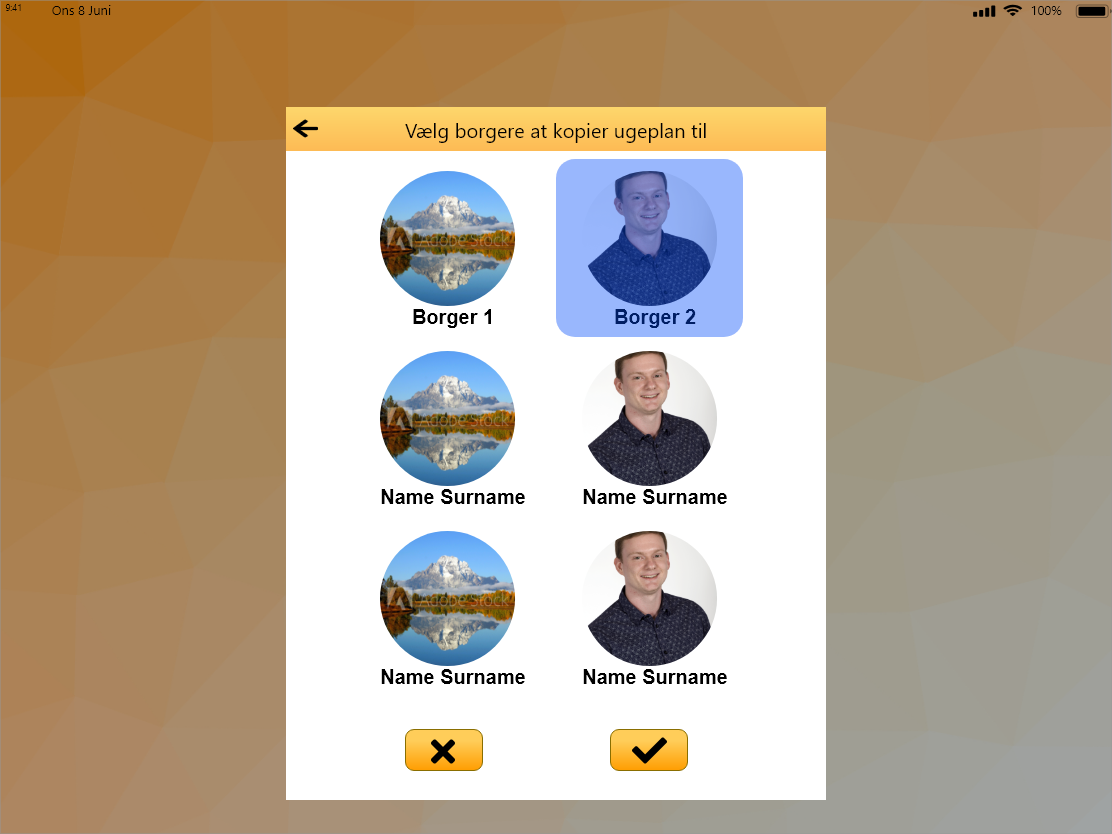
\includegraphics[width=1\linewidth, height=5cm]{sprint3-prototypes/copy_weekplan_confirm_copy.png}
    \caption{Choose citizens to copy weekplan to and confirm}
    \label{fig:copy_weekplan_confirm_copy}
    \end{subfigure} 
\end{figure}
Finally, in \autoref{fig:copy_weekplan_confirmed} we see the confirmation dialog when the weekplan is succesfully copied.
\begin{figure}[H]
    \begin{subfigure}{0.5\textwidth}
    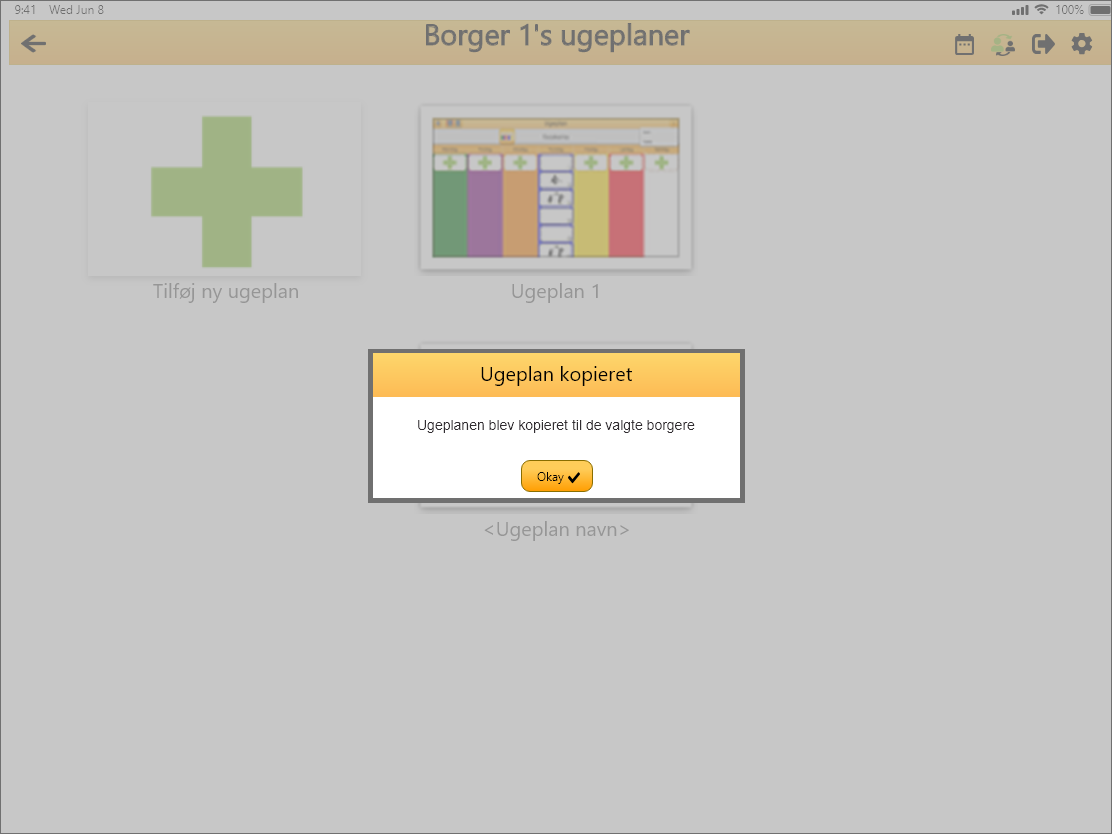
\includegraphics[width=1\linewidth, height=5cm]{sprint3-prototypes/copy_weekplan_confirmed.png} 
    \caption{Weekplan copied confirmation screen}
    \label{fig:copy_weekplan_confirmed}
    \end{subfigure}
\end{figure}

\subsection{Copying of activities}
Here we created two different versions of prototypes that show how activities are copied between weekdays. This is because we were unsure of what the customer would like so we created different versions to show them. The dialog with the checkboxes have the advantage of being able to copy to more than one day at a time.
\begin{figure}[H]
    \begin{subfigure}{0.5\textwidth}
    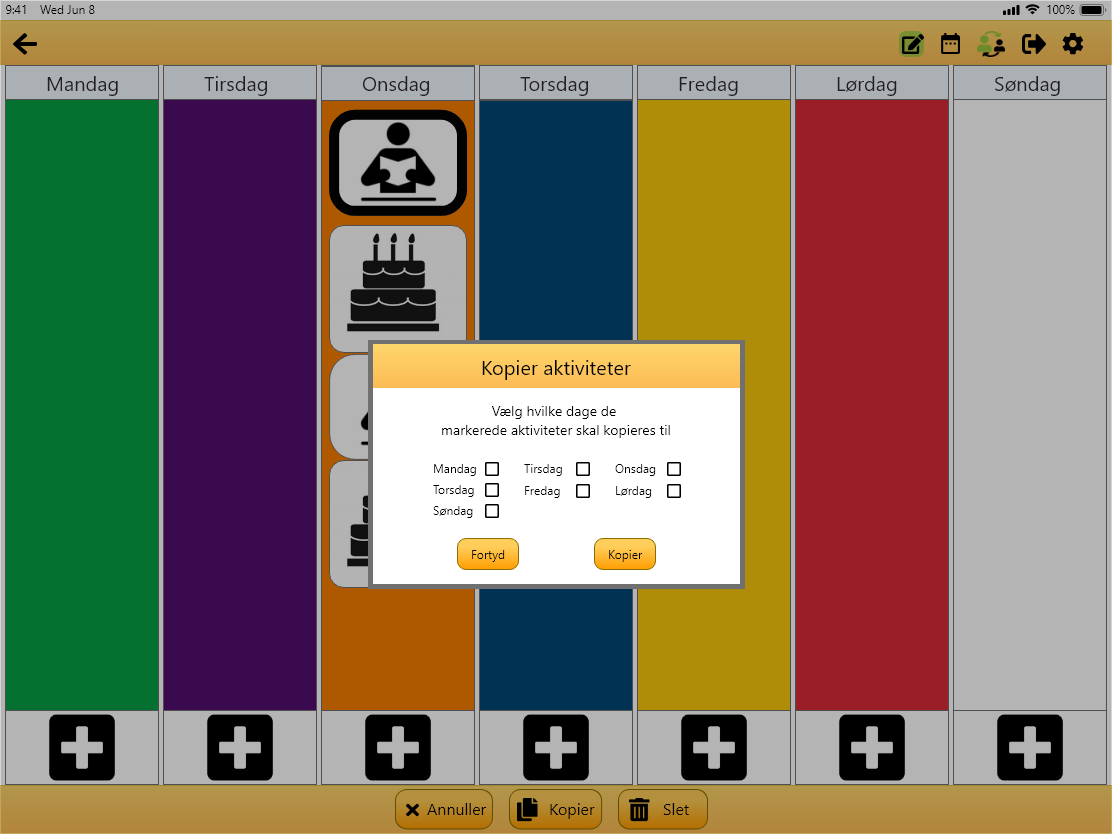
\includegraphics[width=1\linewidth, height=5cm]{sprint3-prototypes/mark_mode_copy_checkbox.png} 
    \caption{Copy activities dialog with checkboxees}
    \label{fig:mark_mode_copy_checkbox}
    \end{subfigure}
    \begin{subfigure}{0.5\textwidth}
        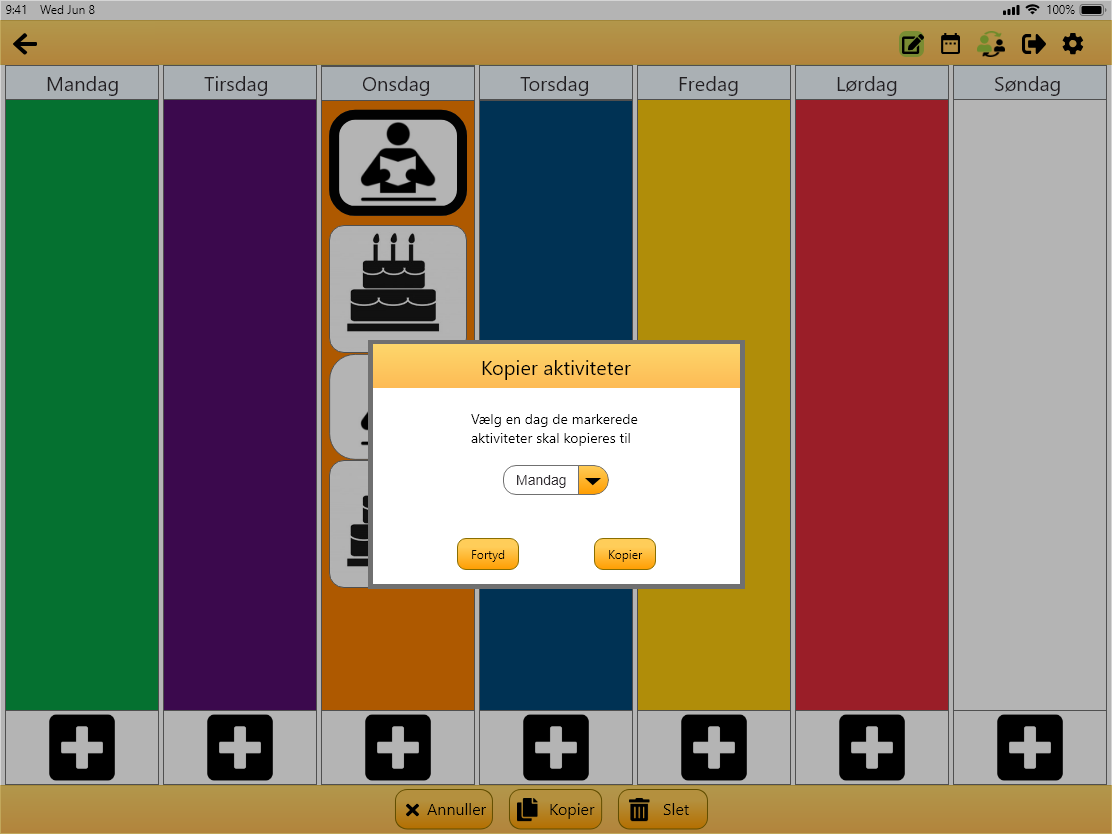
\includegraphics[width=1\linewidth, height=5cm]{sprint3-prototypes/mark_mode_copy_dropdown.png}
    \caption{Copy activities dialog with dropdown}
    \label{fig:mark_mode_copy_dropdown}
    \end{subfigure} 
\end{figure}

\subsection{Adding new pictograms}
The customer would like the option to add their own pictograms if they could not find the one they needed. They suggested being able to add from the gallery of the phone or tablet or by taking a picture directly. So we created a few prototypes this sprint that shows how this could work. First in \autoref{fig:pictogram_bottom_bar} we needed to create a way to go from the pictogram search to a screen where the user could choose pictures from their gallery. A buttom bar with two buttons was enough for this. In \autoref{fig:pictogram_add_gallery} we see the prototype for the screen where you can add photos from the gallery, and enter a name for the pictogram.
\begin{figure}[H]
    \begin{subfigure}{0.5\textwidth}
    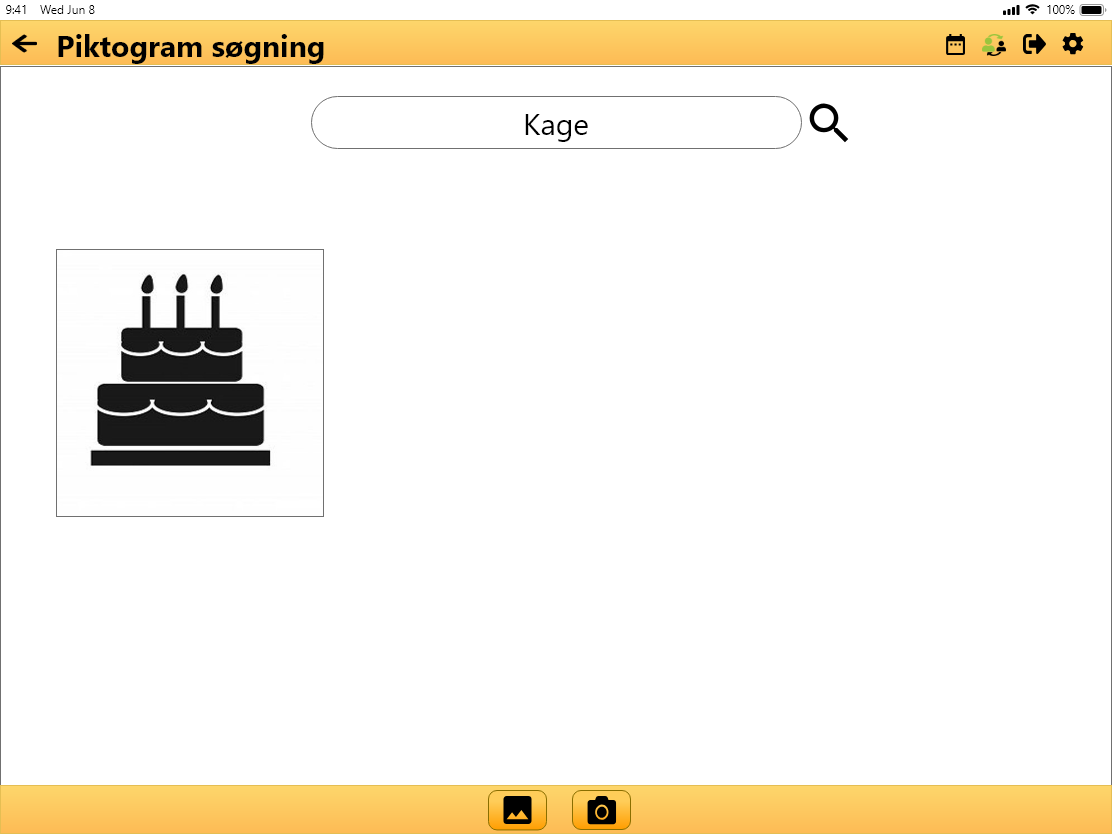
\includegraphics[width=1\linewidth, height=5cm]{sprint3-prototypes/pictogram_bottom_bar.png} 
    \caption{Pictogram search with options in the bottom bar}
    \label{fig:pictogram_bottom_bar}
    \end{subfigure}
    \begin{subfigure}{0.5\textwidth}
        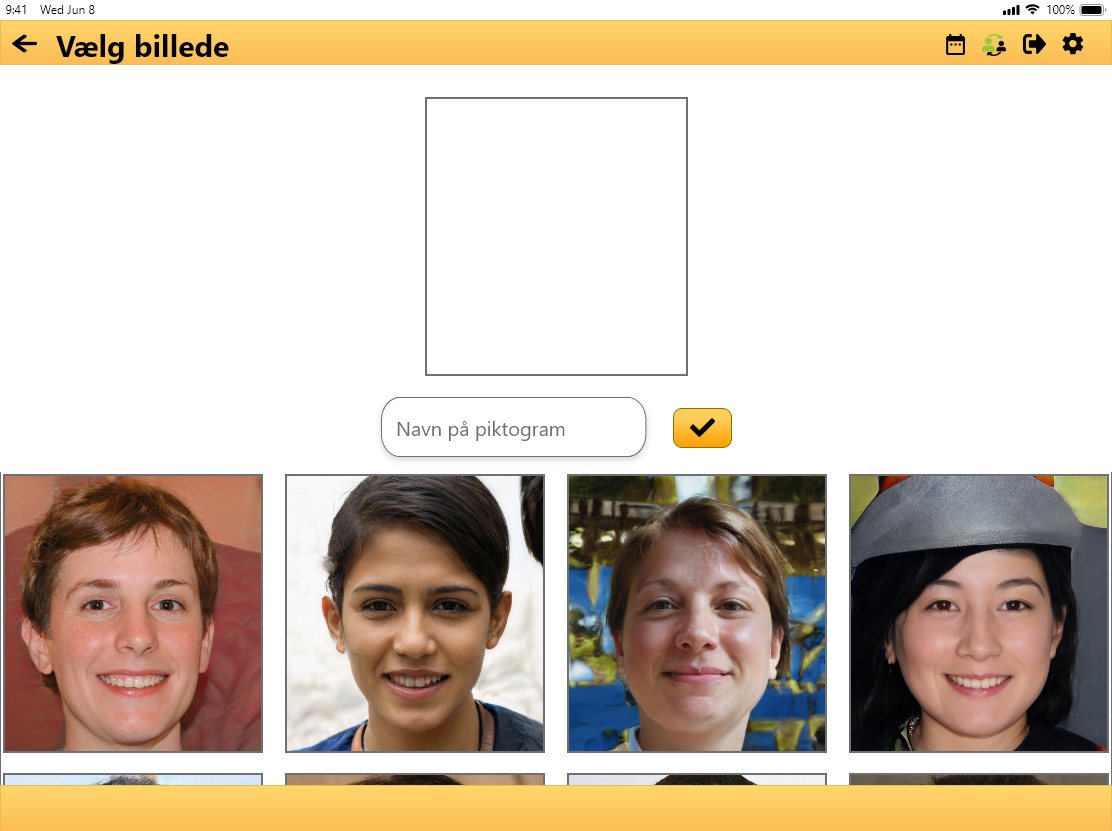
\includegraphics[width=1\linewidth, height=5cm]{sprint3-prototypes/pictogram_add_gallery.png}
    \caption{Screen for adding pictograms from gallery}
    \label{fig:pictogram_add_gallery}
    \end{subfigure} 
\end{figure}
In \autoref{fig:pictogram_add_camera} we see the screen where the user can add a pictogram from the camery, give it name and then add it click the checkmark to save it to the weekplan and in the database.
\begin{figure}[H]
    \begin{subfigure}{0.5\textwidth}
    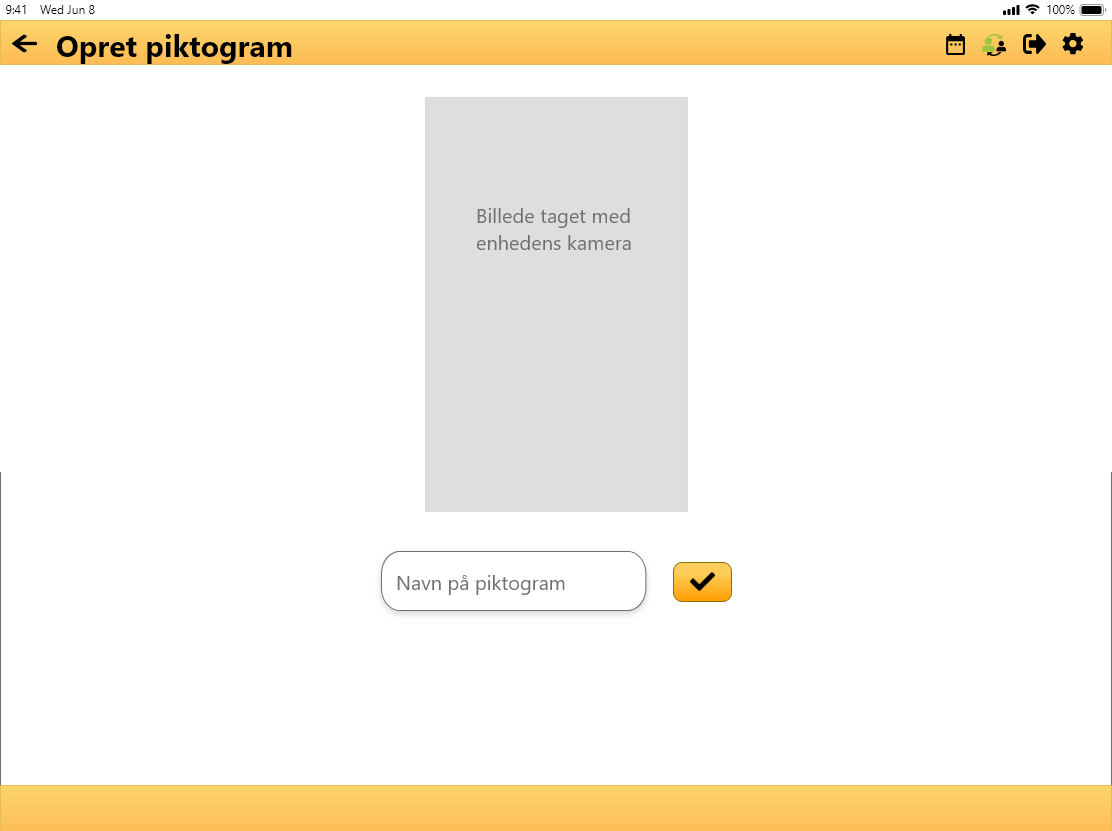
\includegraphics[width=1\linewidth, height=5cm]{sprint3-prototypes/pictogram_add_camera.png} 
    \caption{Screen for adding pictogram by taking a picture with the device}
    \label{fig:pictogram_add_camera}
    \end{subfigure}
\end{figure}